\documentclass{article}
\usepackage{xeCJK,amsmath,geometry,graphicx,amssymb,zhnumber,booktabs,setspace,tasks,verbatim,amsthm,amsfonts,mathdots}
\usepackage{listings,xcolor}
\geometry{a4paper,scale=0.8}   
\title{图论作业 (第四周)}
\author{PB20000113孔浩宇}
\begin{document}
\maketitle
\section*{Ch2}
\subsection*{19.}
\begin{proof}
    设$\nu(T)=\nu$,则$T$中出度为2的顶点数为$\nu -t$,出度为0的顶点数为$t$.
    \begin{enumerate}
        \item [(1)]由二叉树性质有$t=\nu -t+1$.
        \item [(2)]由树性质有$\varepsilon=\nu -1$.
    \end{enumerate}
    \[
        \begin{cases}
            t &= \nu -t+1\\
            \varepsilon &=\nu -1
        \end{cases}
        \ \Rightarrow
        \ \varepsilon=2t-2.
    \]
    即证.
\end{proof}
\subsection*{21.}如图,编码一个符号平均需要二进制数字$3\times 0.25+2\times 0.75=2.25$个.
\begin{figure}[h]
    \centering
    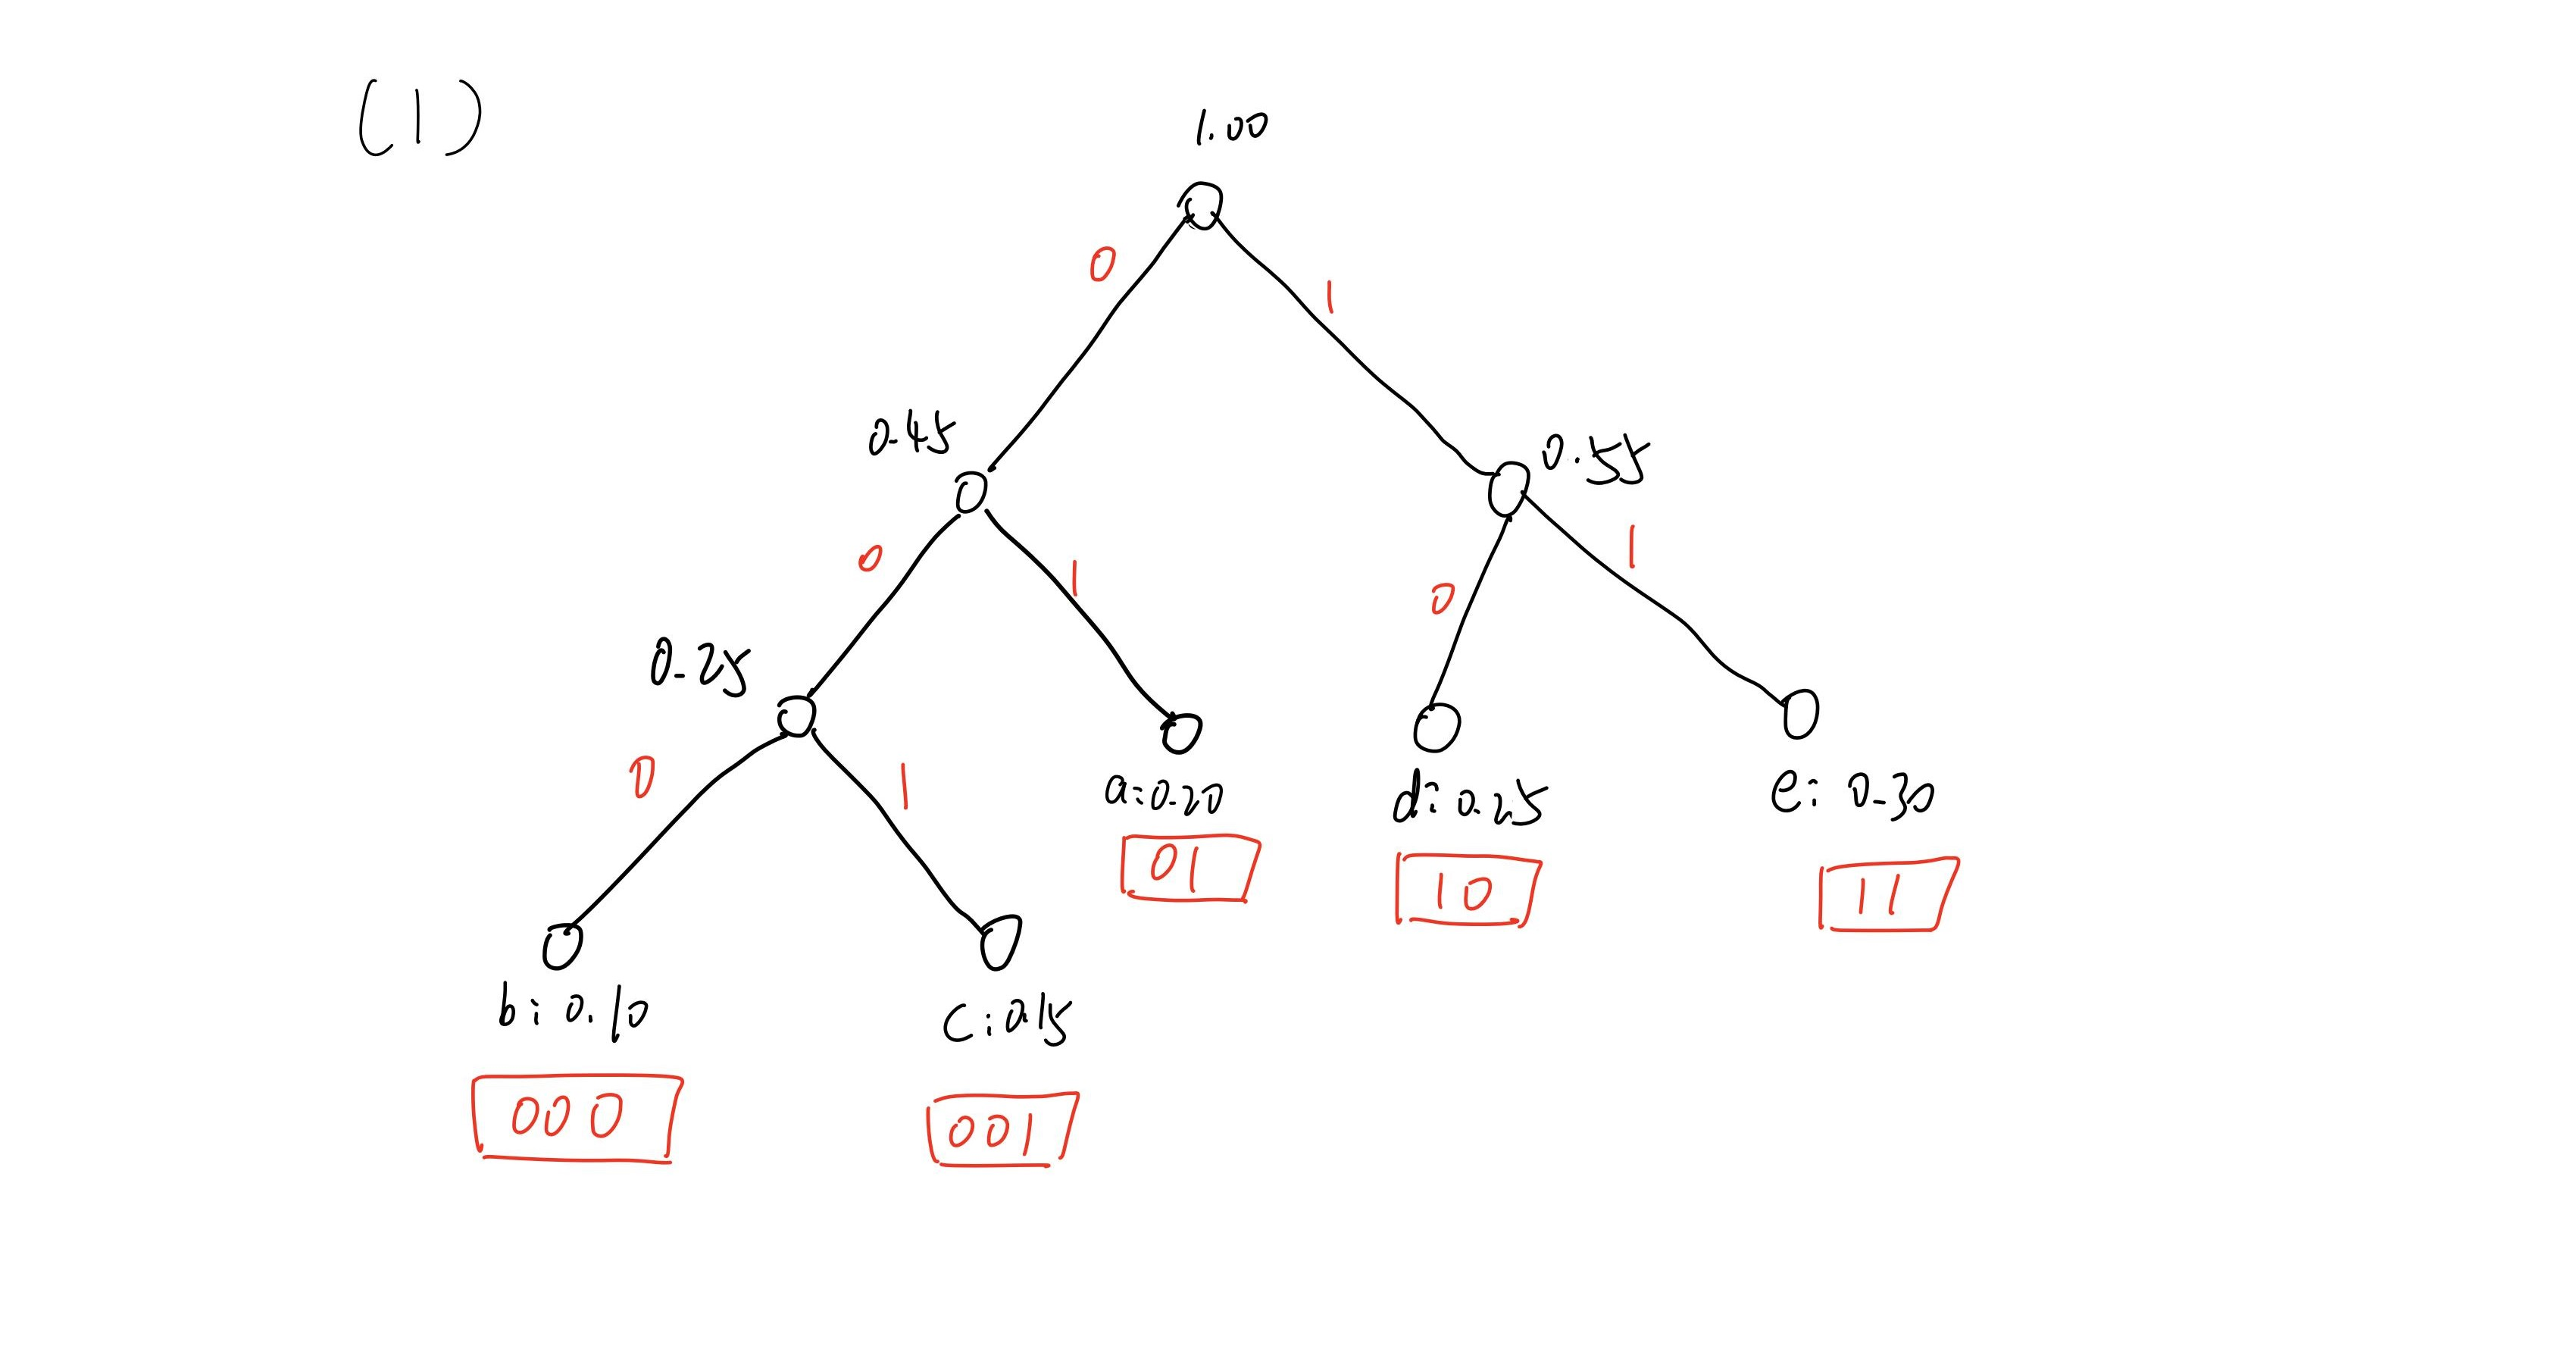
\includegraphics[scale=0.4]{01.jpg}
\end{figure}
\begin{figure}[h]
    \centering
    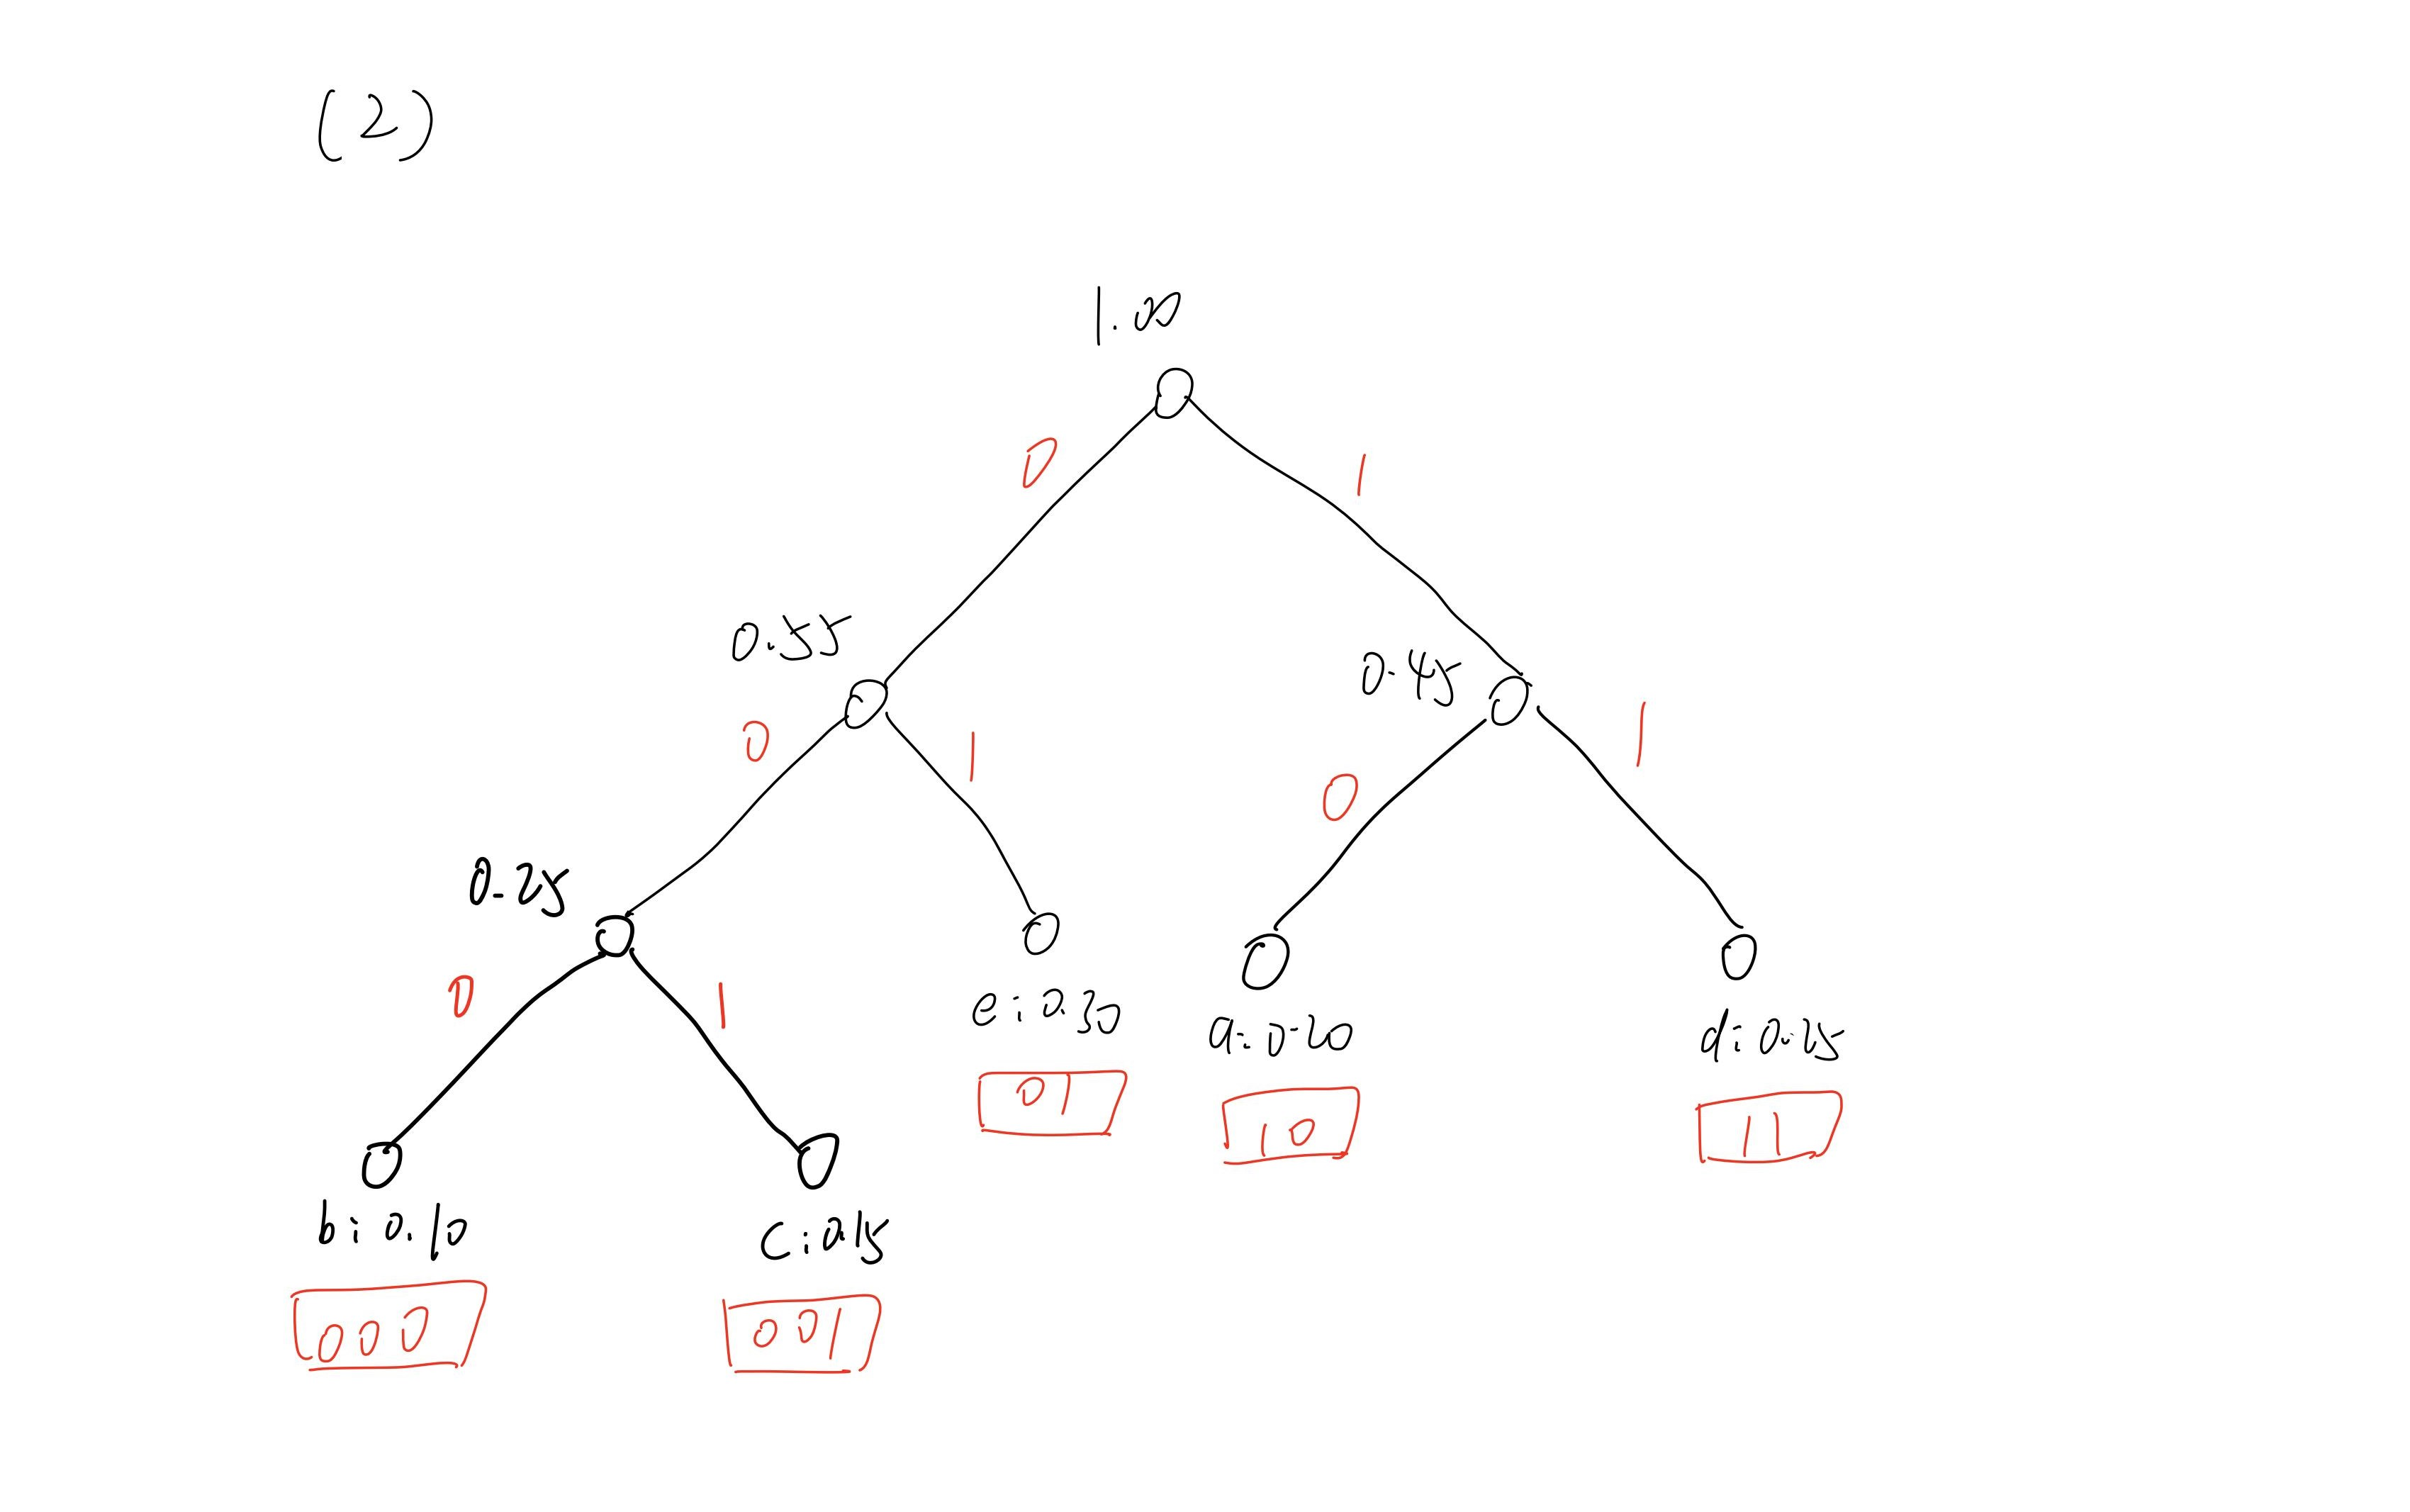
\includegraphics[scale=0.4]{02.jpg}
\end{figure}
\clearpage
\subsection*{24.}
\begin{proof}
    \begin{enumerate}
        \item []
        \item [(1)]记$p_i=2^{-a_i}$,取$A=\max\{ a_i|1\leq i \leq n\},\ K=\{i|a_i=A\}$,记$k=card(K)$,则有
        \begin{align*}
            1=\sum p_i=\displaystyle{\frac{k+\sum\limits_{i\notin K} 2^{A-a_i}}{2^A}}
            \ \Leftrightarrow\ &k+\sum\limits_{i\notin K} 2^{A-a_i}=2^A\\
            \ \Leftrightarrow\ &k=2^A-\sum\limits_{i\notin K} 2^{A-a_i}.
        \end{align*}
        又
        \[
            \forall\ 1\leq i\leq n\ (i\notin K),\ A-a_i\geq 1;\ 
            \Rightarrow\ k\mbox{为偶数};
            \xrightarrow{k>0}\ k\geq 2.
        \]
        即证概率最低$(p=2^{-A})$的消息符号至少有两个,即概率最低的两个消息符号有相同的概率.
        \item [(2)]记Huffman树里顶点权值为$2^{-i}$的顶点的个数为$k_i$.
        
        先证明引理\[\forall\ 1\leq i\leq A,\ k_i \mbox{均为偶数,且}k_i \cdot 2^{-i}=\sum\limits_{a_j\geq i}p_j.\]
        \begin{enumerate}
            \item [(a)]$i=A$,成立.$\ k_A$个权重为$2^{-A}$的顶点两两连接,构成$k_A /2$个权重为$2^{-(A-1)}$的顶点.
            \item [(b)]假设$i=m\ (2\leq m \leq A)$时成立,则
            \[k_m\mbox{个权重为}2^{-m}\mbox{的顶点两两连接,构成}\frac{k_m}{2}\mbox{个权重为}2^{-(m-1)}\mbox{的顶点}.\]
            此时有
            \begin{align*}
                &k_{m-1}\cdot 2^{-(m-1)}=\frac{k_m}{2} \cdot 2^{-(m-1)}+\sum\limits_{a_i=m-1} p_i=k_m\cdot 2^{-m}+\sum\limits_{a_i=m-1}p_i=\sum\limits_{a_i\geq m-1}p_j\\
                \Rightarrow\ &k_{m-1}\cdot 2^{-(m-1)}+\sum\limits_{a_i<m-1} p_i=\sum p_i=1\\
                \Rightarrow\ &k_{m-1}\mbox{为偶数}.
            \end{align*}
        \end{enumerate}
        综合$(a)(b)$,即证\[\forall\ 1\leq i\leq A,\ k_i \mbox{均为偶数,且}k_i \cdot 2^{-i}=\sum\limits_{a_j\geq i}p_j.\]
        由上推理过程可知,Huffman树里顶点权值的取值有且仅有$2^{-i}(0\leq i\leq A)$,且
        \[
            \omega(u)=2\cdot\omega(v)\Leftrightarrow L(v)=L(u)+1.
            \xrightarrow{\omega(v)=\frac{1}{2},L(v)=1}
            \omega(v)=2^{-i} \Leftrightarrow L(v)=i.
            \Rightarrow L(v)=-\log_2 \omega(v).
        \]
        由此可得
        \[
            WPL=\sum \omega_i L_i=\sum p_i\cdot \left(-\log_2 p_i \right)=-\sum p_i \log_2 p_i .
        \]
        即证.
    \end{enumerate}
\end{proof}

\end{document}
